\chapter{Introduction}
\label{secIntro}

\linnet{} is an application to compute the transfer function of linear,
electronic circuits. The computation is done symbolically, not
numerically, and the result is a formula rather than a number or a series
of such. The found formula is the Laplace transform of the dependencies of
the voltages and currents in the circuit on the input voltages and
currents.


% Locally define a figure representation specific to the table.
{
\newcommand{\incTabFig}[2]{\includegraphics[width=#2]{#1}}

% This define is related to the specifics of the array package; see
% http://texwelt.de/wissen/fragen/3401/zentrieren-text-in-tabelle (as of
% July 25 2014) for more
\newcolumntype{M}[1]{>{\centering\arraybackslash}m{#1}}

\begin{table}[t]
\begin{center}
\begin{tabular}{|l|c|M{2cm}|}

\hline

% The column headers:
Device                               & ID          & Symbol                        \\
\hline

\hline

% Table entries start here.
%   The raisebox command is used to avoid a hiding overlap of the topmost
% figure with the header separating line.
\raisebox{0pt}[15pt][0pt]{Resistor}  & \code{R}    & \incTabFig{deviceR}{1.9cm}    \\ 
Conductance                          & \code{Y}    & \incTabFig{deviceY}{1.9cm}    \\
Capacitor                            & \code{C}    & \incTabFig{deviceC}{0.8cm}    \\ 
Inductivity                          & \code{L}    & \incTabFig{deviceL}{2cm}      \\ 
Ideal operational amplifier (op-amp) & \code{OP}   & \incTabFig{deviceOP}{1.3cm}   \\ 
Constant voltage source              & \code{U}    & \incTabFig{deviceU0}{1cm}     \\
Voltage controlled voltage source    & \code{U(U)} & \incTabFig{deviceU(u)}{1cm}   \\
Current controlled voltage source    & \code{U(I)} & \incTabFig{deviceU(i)}{1cm}   \\
Constant current source              & \code{I}    & \incTabFig{deviceI0}{0.4cm}   \\
Voltage controlled current source    & \code{I(U)} & \incTabFig{deviceI(u)}{0.4cm} \\
Current controlled current source    & \code{I(I)} & \incTabFig{deviceI(i)}{0.4cm} \\
Current probe (wire)                 & \code{PI}   & \incTabFig{devicePI}{1.8cm}   \\ \hline
\end{tabular}
\caption{Supported linear devices}
\label{tabSupportedDevices}
\end{center}
\end{table}
} % End of local scope of \incTabFig

A linear electronic circuit is a combination of the supported basic
devices as listed in table \ref{tabSupportedDevices}. The circuit is input
to \linnet{}. The representation of the circuit is a list of devices with
connectivity information. The interconnections are expressed by references
to nodes, where a node is a point of the circuit, which normally at least
two devices are connected to. This leads to a simple formal syntax, the
circuit network list. This list can be created and maintained with a text
editor; there's no graphical interface for editing a circuit.

\begin{figure}
\centering
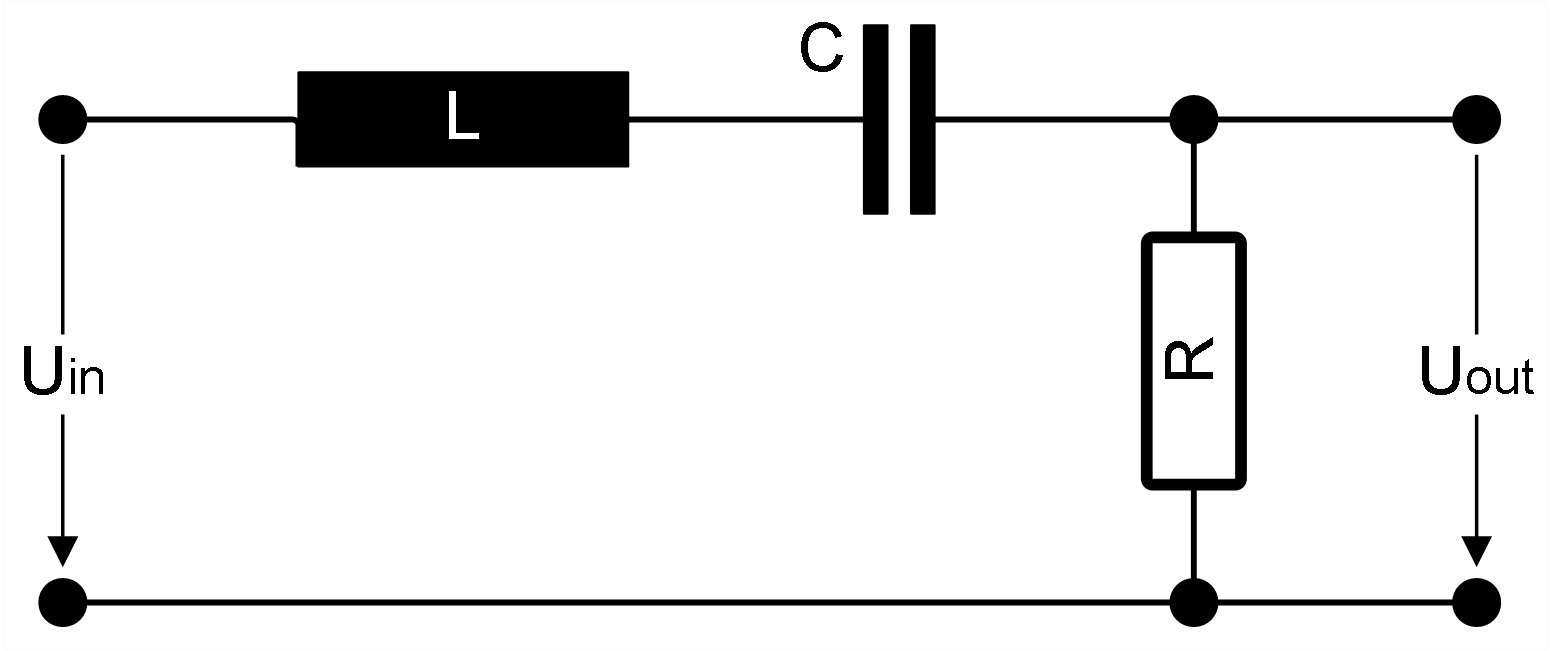
\includegraphics[width=5.29cm]{FirstIntroExample}
\caption{Simple example of a linear electronic circuit}
\label{figFirstIntroExample}
\end{figure}

The computed formulas are printed to the console and to the application
log file and can be used for further investigation or for publications or
didactic purpose.

To make the application somewhat more attractive it exports the computed
formulas as Octave or MATLAB script code, too. Numeric evaluation becomes
a simple one-line command in Octave. The formulas are exported as LTI
transfer function objects so that the complete set of analysis functions
from the Octave control toolbox can be applied just like that. This
reaches from simple transfer function plotting to stability analyses and
system response computation on arbitrary system input.

Please refer to figure \ref{figFirstIntroExample} as an example
of how \linnet{} works. This is a simple RLC element with a transfer
function of second order. It can be represented by the following circuit
netlist:
\begin{verbatim}
U Uin in  gnd
L L   in  K1
C C   K1  out
R R   out gnd
PLOT G U_out U_in
\end{verbatim}
Given this was put into file rlc.cnl, then we can run \linnet{}:
\begin{verbatim}
linNet -o rlc.cnl
\end{verbatim}
%\clearpage
and would yield the output:
\begin{verbatim}
User-defined result G (Bode plot):
The dependency of U_out on U_in:
  U_out(s) = N_U_out_U_in(s)/D_U_out_U_in(s) * U_in(s), with
    N_U_out_U_in(s) = R*C * s
    D_U_out_U_in(s) = L*C * s^2
                      +R*C * s
                      +1
\end{verbatim}

\begin{figure}
\centering
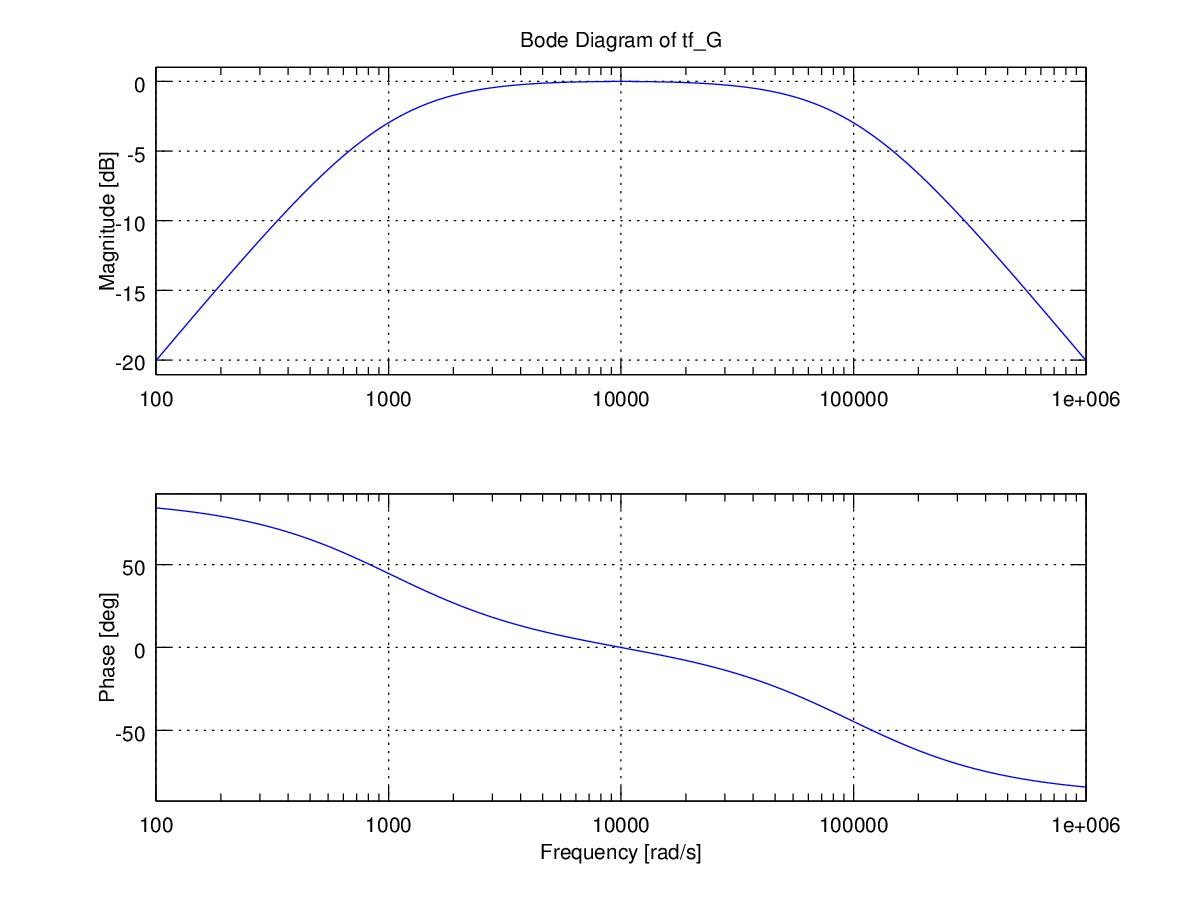
\includegraphics[width=0.7\textwidth]{FirstIntroExample_OctaveOutput}
\caption{Octave plot of transfer function of the system in figure
\ref{figFirstIntroExample}}
\label{figFirstIntroExample_OctaveOutput}
\end{figure}

Going to Octave and typing \code{G} to plot the transfer function (still
using default device values) gives us figure
\ref{figFirstIntroExample_OctaveOutput}. More plots or plots with altered
device values are a matter of single commands in Octave.

\linnet{} means ``linear network''. It founds on a symbolic solver for
linear equation systems. There's no way to model any non linear effects
like noise, voltage or current limits, non-linear distortions or switching
operations. All of these effects play an important role in real electronic
circuits and a good deal even uses these effects as their principle of
operation -- you won't find \linnet{} helpful for an investigation of
these kind of effects or circuits. There are many numeric circuit
simulation tools, which are capable to do this, in the first place the
popular open source tool SPICE with all its derivates. \linnet{} is
conceptually not a competitor of these tools, although it can behave a
tiny bit alike when using Octave as numeric post-processor. \linnet{} is
not the worse SPICE, \linnet{} is different.